\section{Background}
\label{sec:background}

\subsection{Domain-Specific Languages}

Like general purpose languages, domain specific languages are specified in terms of three interdependent dimensions: abstract syntax, concrete syntax, and semantics \cite{Harel:2004b}. The \textit{abstract syntax} refers to the structure of the DSL expressed as the set of concepts that are relevant to the domain and the relationships among them. The \textit{concrete syntax} refers to the association of the language concepts to a set of symbols (either graphical or textual) that facilitate the usage of the DSL. These representations are usually supported by editors that allow users to write programs using the symbols defined by the concrete syntax acting as the graphical user interface of the DSL. Finally, the \textit{semantics} of a DSL refers to the meaning of its domain concepts. This meaning is expressed through static constraints and dynamic behavior specification. The static constraints usually correspond to the type system of the DSL. In turn, the dynamic behavior defines the manner in which domain concepts are manipulated at runtime, typically through the definition of an interpreter or compiler.

In this paper we are interested in executable DSLs which abstract syntax is specified by means of metamodels and semantics is specified operationally as a set actions (or methods) on the metaclasses of the metamodel. We adopt the vocabulary presented in \cite{Combemale:2013} and we term these actions as \textit{domain-specific actions} (DSAs). The concrete syntax is out of the scope of this paper. 

%A DSL is specified in terms of its abstract syntax, concrete syntax and semantics. There is a mapping between the concrete syntax and the semantics. Then, a DSL specification can be defined as triple $<AS, CS, Sem>$.

\subsection{On the notions of \textit{commonalities} and \textit{potential reuse} in DSLs}

As aforementioned, a DSL is intended to focus on a specific aspect of the system under construction. Due to the complexity of current systems, there is a large amount of concerns to deal with. As a result, there is a proliferation of DSLs in the literature \cite{Mernik:2005b}. Although many of those existing DSLs are completely different and with independent domains; it is also true that we can find related DSLs with overlapping domains. Moreover, there are set of DSLs for which the domains can be hierarchically organized \cite[p. 60-61]{voelter:2013}.

Figure \ref{fig:domains} illustrates the situation explained above. At the left of the figure there are two DSLs that are totally independent. That means that they do not share any of their domain abstractions, and consequently, there is not potential reuse between them. Differently, the two DSLs shown in the center of the figure have overlapping domains. That means that there are a subset of domain abstractions that are \large\textbf{``equal'' }\normalsize in both languages. In such case, we say that the domains abstractions are shared by the two DSLs and that the domains overlap. Note that because domain abstractions are defined in the specification of the two DSLs, it is natural to thing that the definitions are equal. That means that those definitions are replicated in the specifications of the DSLs. Thus, there is potential reuse. The case presented at the right of the figure is even more interesting. In that case there is a DSL that contains all the domain abstractions of another DSL. In the vocabulary introduced in \cite[p. 60-61]{voelter:2013} that means that there is a domain hierarchy i.e., the domain of the DSL 1 is a subdomain of the domain of the DSL 2. In that case, there is potential reuse because in the sense that the DSL 2 could import the DSL 1 as part of its specification without having to redefine all those domain abstractions. 

\begin{figure}
\centering
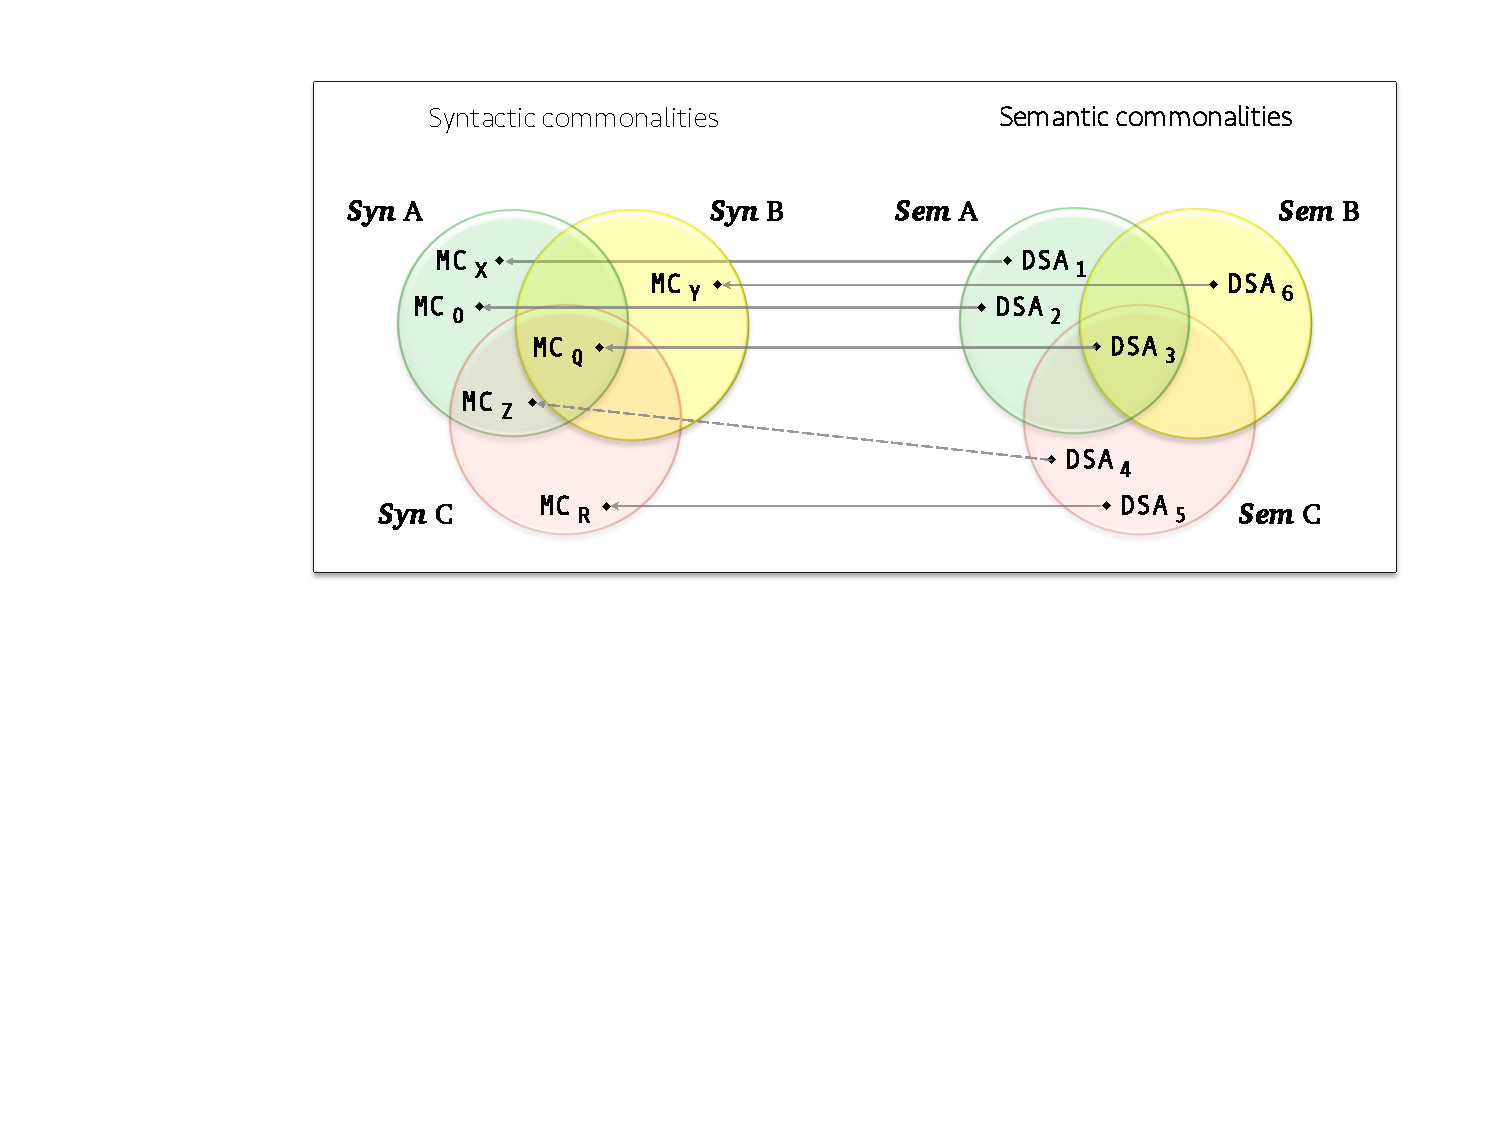
\includegraphics[width=1\linewidth]{images/domains-fig.pdf}
\caption{Commonalities between domains and potential reuse}
\label{fig:domains}
\end{figure}

\subsection{Equivalence between language constructs}

So far, we have based the notion of potential reuse in DSLs on the commonalities existing in the specification of a set of DSLs. Nevertheless, this supposes that we are able to compare two language constructs in order to know whether their specifications are equivalent. The comparison of two language constructs relies on two dimensions: (1) comparison of the meta-classes in the abstract syntax; and (2) comparison of the domain-specific actions in the semantics. The reminder of this section is dedicated to explain this notion of equality for both meta-classes and DSAs.

\vspace{-2mm}
\subsubsection{Comparing meta-classes.} A first approach to compare meta-classes is by comparing their name. Two meta-classes are equal if they have the same name. This approach results quite useful if we consider that, in most of cases, the name of the meta-class refers to a domain concept and it is quite probable that, we can find potential reuse. Unfortunately, comparison of meta-classes by using only their names might have some problems. There are cases in which two meta-classes with the same name are not exactly the same. This may occur either because they not refer to the same language construct or because one meta-class is more specialized than the other one. In such cases, an approach that certainly helps is to compare meta-classes not only by their names but also by their attributes and references. Although this second approach might be too restrictive, it implies that the specification of the two meta-classes are exactly the same so potential reuse is guaranteed.

\vspace{-2mm}
\subsubsection{Comparing domain-specific actions.} Intuitively, the comparison of two domain-specific actions can be performed by checking if their signatures are equal. This approach is practical and also reflects potential reuse; one might think that the probability that two domain-specific actions with the same signatures are the same is elevated. However, as the reader might imagine, there are cases in which signatures comparison is not enough. Two domain-specific actions can perform different computations even if they have the same signatures. As a result, a second approach for comparing DSAs relies in the comparison of the body of the operations. Note that comparing the body of the operations can be arbitrary complex task. Indeed, if we try to compare that the actions are semantically equivalent we rely on the semantic equivalence problem that, indeed, is known as be undecidable. In this case, we prefer a more conservative approach and we only compare the structure of the DSA. We use the approach proposed in X. Basically, it accepts operations with the same structure and permits certain differences. Concretely, names of variables and parameters can change.

\vspace{-2mm}
\subsubsection{Semantical variability.} A necessary condition for deciding whether two language constructs are equivalent is that both, the meta-class and the domain-specific actions are equivalent. This guarantees that the specification is the same not only at the level of the abstract syntax but also at the level of the semantics. However, there is a phenomenon in the literature that corresponds to semantical variability. There is semantical variability when there there are two constructs that having the same abstract syntax (i.e., their meta-classes are equal) differ in the domain-specific actions. This case is of interest for us because even in the presence of semantical variability we can have some potential reuse. If the meta-classes of two constructs are the same we can reuse them even if their domain-specific actions are different. 
